\documentclass[a4paper,10pt]{article}
% Use ctrl + alt + V to view live pdf

% Packages
\usepackage[utf8]{inputenc} % For encoding
\usepackage[T1]{fontenc} % Better handling of accented characters and hyphenation
\usepackage{microtype} % Improves spacing and justification
\usepackage{amsmath, amssymb} % For equations and symbols
\usepackage{graphicx} % For including graphics/images
\usepackage{caption} % For customizing figure and table captions
\usepackage{subcaption} % For subfigures and subcaptions
\usepackage{float} % For fixing figure and table positions
\usepackage{booktabs} % For professional-looking tables
\usepackage{siunitx} % For consistent typesetting of units and numbers
\usepackage[margin=2cm]{geometry} % Adjusts page margins
\usepackage{fancyhdr} % For custom headers and footers
\usepackage{lmodern} % For a professional-looking font (main body font)
\usepackage{titlesec} % For title customization
\usepackage{array} % For custom table formatting
\usepackage[colorlinks=true, linkcolor=black, urlcolor=black]{hyperref} % Colored links without boxes
\usepackage{cleveref} % For improved cross-referencing    
\usepackage{multirow}
\usepackage{enumitem}
\usepackage{listings}
\usepackage{xcolor}
\usepackage{textcomp}
\usepackage{tabularx}
\usepackage{changepage}
\usepackage{tikz}
\usepackage{pdfpages}
\usetikzlibrary{shapes.geometric, arrows}
\newcolumntype{Y}{>{\centering\arraybackslash}X}
% Reduce spacing before and after \section
% \titlespacing{\section}{0pt}{1.0em}{0.5em}
% Reduce spacing before and after \subsection
% \titlespacing{\subsection}{0pt}{0.8em}{0.3em}


\lstdefinestyle{verilog-style}{
    language=Verilog,
    basicstyle=\ttfamily\footnotesize,
    keywordstyle=\bfseries\color{blue},
    commentstyle=\itshape\color{gray},
    stringstyle=\color{red},
    numbers=left,
    numberstyle=\tiny\color{gray},
    stepnumber=1,
    breaklines=true,
    showstringspaces=false,
    frame=single
}
\lstset{style=verilog-style}
\lstset{captionpos=b}
\lstset{basicstyle=\ttfamily\scriptsize} 
\renewcommand{\lstlistingname}{Program}

% Custom settings
\pagestyle{fancy}
\fancyhf{}
\fancyhead[L]{\textit{GB3 - Risc-V Processor}} % Header left
\fancyhead[R]{\textit{Will Hewes - wh365}} % Header right 
\fancyfoot[C]{\thepage} % Footer center
\setlength{\headheight}{15pt} % Header height
\setlength{\parindent}{0em} % Indentation for paragraphs
\setlength{\parskip}{0.2em} % Add spacing between paragraphs
\setlength{\abovedisplayskip}{0.5em}
\setlength{\belowdisplayskip}{0.5em}
\setlength{\abovedisplayshortskip}{0.5em}
\setlength{\belowdisplayshortskip}{0.5em}
\setlist{topsep=0em, partopsep=0em, itemsep=0em, parsep=0em}

\graphicspath{{Images/}}

% \renewcommand{\arraystretch}{1.2}

% Title formatting
\renewcommand{\maketitle}{
    \begin{center}
        \LARGE \textbf{ENGINEERING TRIPOS PART IIA} \\ 
        \vspace{0.5em}
        \Large \textbf{GB3 - Risc-V Processor} \\ 
        \vspace{0.5em}
        \textbf{Final Report} \\
        \large Group 4 - Resource Usage \\
        \vspace{1em}
        \large Will Hewes - wh365 \\ 
        Pembroke College \\ 
        \vspace{0.5em}
    \end{center}
}

\begin{document}
\pagenumbering{gobble}
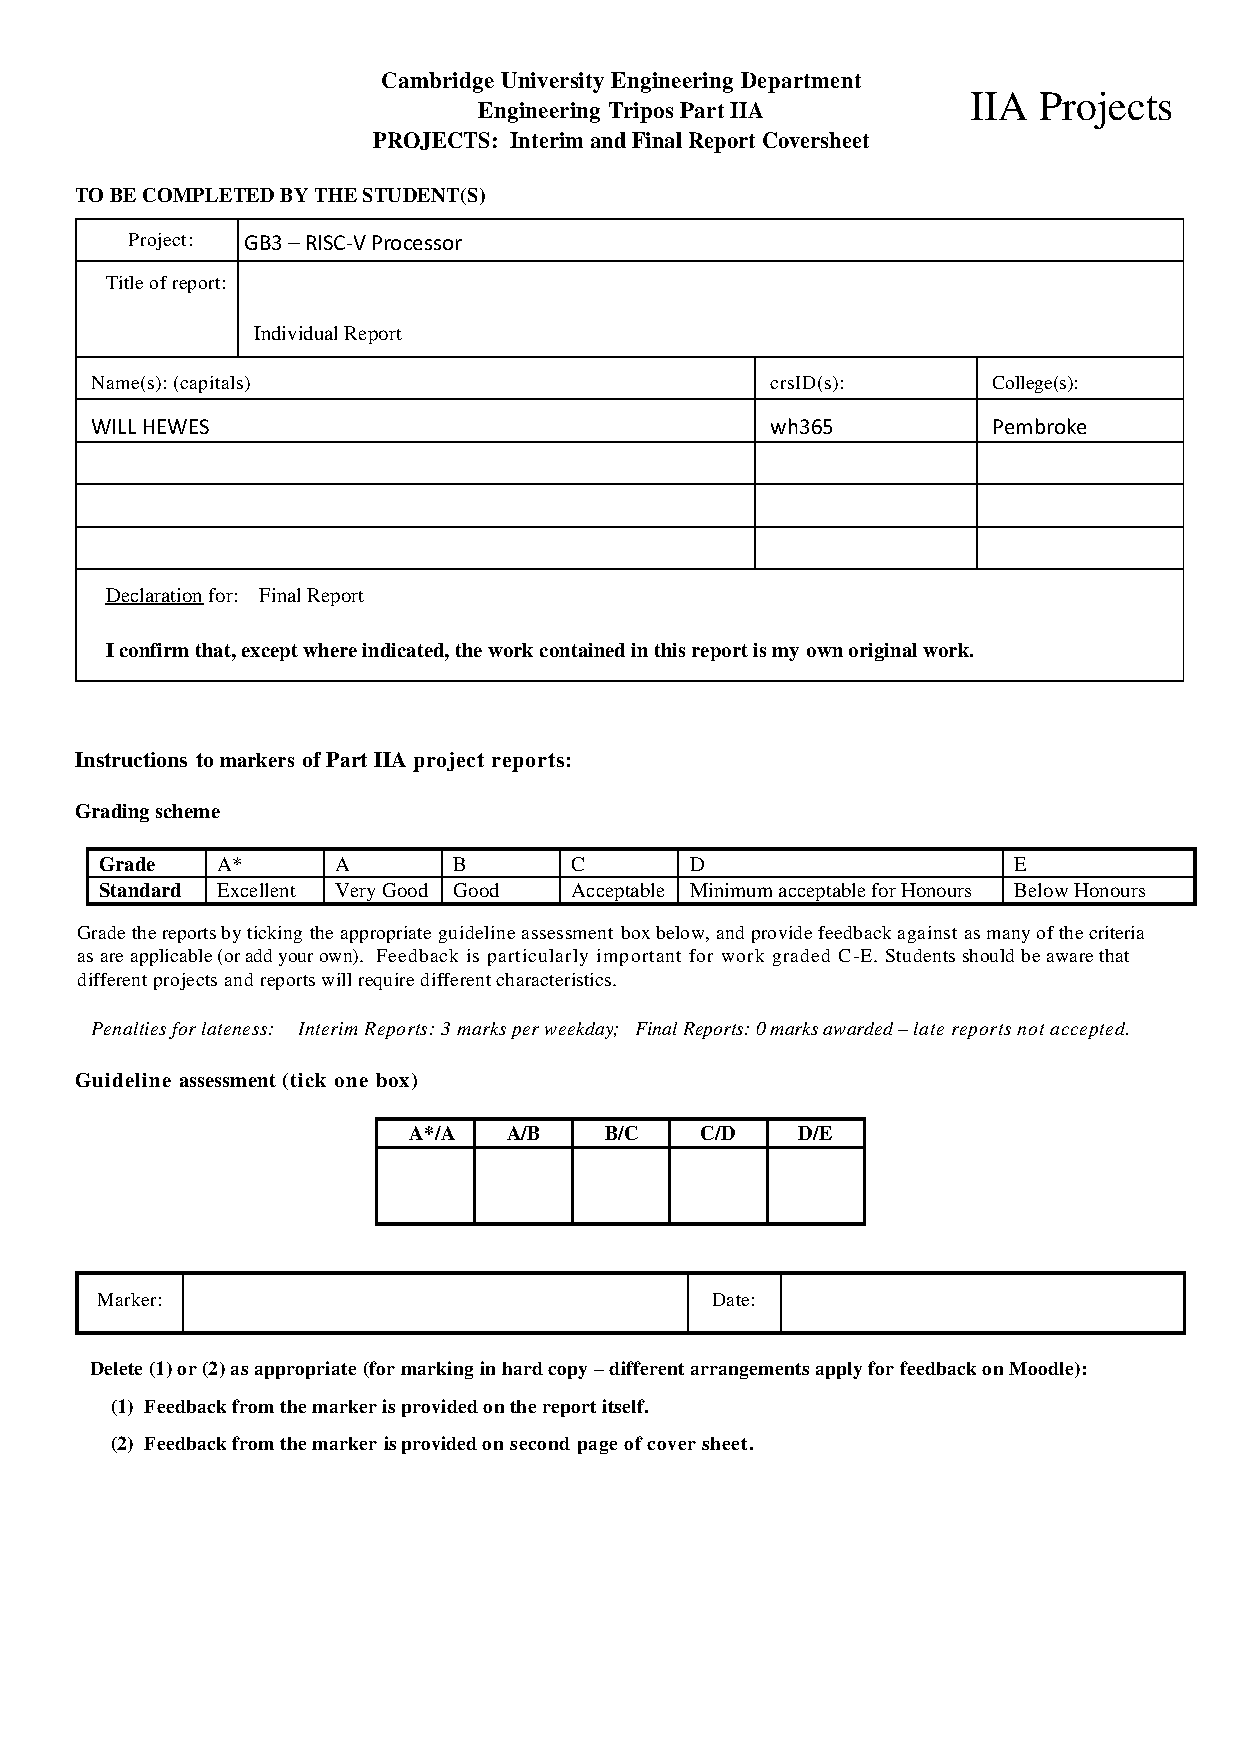
\includepdf[pages=-]{Handouts/IIA Project Coversheet Feedback Final Report.pdf}
\maketitle
\hrule
\tableofcontents
\newpage
\pagenumbering{arabic} \setcounter{page}{1}
% No more than 8 A4 sides, excluding appendices
% Include tables and descriptions in resource usage?

\section{Introduction}
\label{sec:Introduction}
% This section should give a detailed introduction to the changes
% you have implemented for your role on the team 
% (1 A4 side)

This project involves the collaborative design and implementation 
of a RISC-V processor on an iCE40 FPGA device. 
The overarching aim is to optimise 
the processor design with respect to its 
performance, power dissipation, and resource usage, 
while balancing trade-offs between these three aspects. 
Each team member is responsible for focusing on one of the three aspects
and my reports focus on the resource usage of the design.
This report is the final report for this project.

In the first report we evaluated three programs as a baseline against
which our improvements could be compared.
The first of these three porgrams was \texttt{hardwareblink},
a program which relied purely on combinational and sequential logic
to blink an LED on the FPGA,
bypassing the processor core entirely. 
As a result it had very low resource utilisation across the board.
The second program evaluated was \texttt{softwareblink},
which performed the same task but instead implemented through software,
utilising the sail-core processor.
As a result, the design used a much larger number of logic cells,
and also introduced the usage of a few other primitive cells such as 
block RAMs and DSP blocks.
The final program was \texttt{bubblesort}, which would perform a 
bubblesort algorithm and blink the LED to confirm it was finished.
Due to the increased complexity of the program,
the logic cell utilisation was greater than for \texttt{softwareblink},
but crucially the other primitives did not increase, 
as they relied primarily on their design within the verilog files.
The final test would be to process 
a new, unseen program under our implementation and evaluate it for its 
resource usage, performance and power dissipation.
As such we chose to base our testing primarily 
on the more complex \texttt{bubblesort},
allowing us to push the processor further,
offering a more representative view of our design.
It should be noted the other programs were still tested
to ensure functionality and check progress,
they were just less emblematic of our implementaions capabilities.

The baseline implementation on the FPGA showed several inefficiencies 
in its core design and made poor use of 
some of the resources available on the board. 
Before describing the changes made, it's helpful to briefly explain 
what those resources are and how they affect the processor.

Logic cells, or LCs, are the basic building blocks used to 
implement logic on the FPGA. 
They include components like look-up tables and flip-flops, 
and are used for almost everything, including 
arithmetic, control signals, and registers. 
Because almost everything in the design depends on logic cells in some way, 
reducing how many are used was the main goal throughout the project.
The changes that directly improved LC usage primarily came from
cleaning up registers, wires, and other redundant logic where possible.
One noteable example of this was reducing a multiplexing wire signal
from 32 bits down to 11 bits. These examples will be discussed in more detail
in the body of the report.

Other primitives available on the board are similarly powerful,
though they have a key difference - they are fixed for a given implementation
on the microprocessor.
This means that whereas LCs will increase and potentially become limiting
for a particularly complex program, 
other primitives such as block RAMs, DSP registers, and buffers
will not increase outside of the capacity of the board if designed properly.

Block RAMs are small dedicated memory blocks built into the FPGA. 
They're useful when a design needs to store more data 
than would be practical with flip-flops alone. 
In the baseline implementation, 
they were used by certain parts of the processor 
such as the register file and CSR logic. 
By removing CSR logic from the design,
the number of block RAMs used was reduced 
from 20 to 12 of the 30 available,
meaning that more memory functions could be moved to the RAM 
in order to preserve logic cells.
Unfortunately these changes could not be implemented due to time constraints,
but the plan was to ...

DSP blocks are specialised units designed for fast arithmetic. 
Instead of building adders and multipliers out of regular logic, 
the FPGA provides a few dedicated DSP blocks that are faster and use less space. 
The baseline design didn't use any of these, 
relying entirely on logic cells even for basic addition. 
One of the most significant alterations to the base implementation
was forcing the \textit{adder.v} to make use of these DSP blocks
for addition and subtraction, 
freeing up LUTs to be used in more sophisticated logic.
Implementing this change reduced the LC usage by ..., 
at the expense of 3 of the 8 DSP blocks available,
leaving room for further improvement in this regard.

In addition to these changes that were successfully implemented,
there are many that ...

\newpage

\section{Design Strategy}
\label{sec:Design_Strategy}
% Describing the specific design strategy employed for your role in the team (0.5-1 A4 side)
% Timeline diagram?
% Include subsection on the baseline processor, both description of its structure and resource usage

As I was initially unfamiliar with processor and FPGA design at this level, 
the early stages of the project were spent working through the course material 
and exploring online resources to build a clearer understanding of 
where changes could be most effectively targeted. 
This initial research was followed by a series of small, 
hands-on changes to the Verilog code, 
helping build familiarity with the processor's structure and behaviour.
In hindsight, these early edits were made 
without a broader design strategy in place, 
but they laid the groundwork for a more focused and informed optimisation approach 
that developed as the project progressed.
This unstructured approach naturally led to a few early mistakes, 
such as unintentionally breaking functionality or introducing hard-to-trace bugs.
These mistakes will be discussed more in Section \ref{sec:Problems_Encountered}.
These issues highlighted the need for a more disciplined workflow, 
which later included stricter version control, 
more careful integration with other modules, 
and simulations to verify that signals behaved as expected after changes.

As a team we worked together through git, allowing us to collaborate effectively.
We set up different branches from the \texttt{main} for each of us to use, 
with the plan being that we would work on some changes independently 
and then merge our changes cohesively.
My workflow initially consisted of running the various \texttt{Makefile}
commands to initiate yosys and nextpnr, 
synthesising our implementation and performing a place-and-route operation.
I saved the reports from these operations to a .txt file, 
allowing me to perform \textit{git diff} on the text file 
from any of my commits to easily see the impact that each change had 
on various elements of resource usage, as well as timing.
I used a single command block to automate this workflow 
to rapidly implement and track my changes, 
which is shown below in Program \ref{prog:Workflow}.

\begin{lstlisting}[language=bash,
    caption={Workflow used to synthesise and record results},
    label={prog:Workflow}]
make clean && \
make && \
make install && \
cd ../processor && \
make > Resources.txt 2>&1 && \
cd ../bubblesort
\end{lstlisting}

This proved instrumental to a quick and iterative development cycle, 
allowing me to synthesise, place-and-route, and record results in a single step.
This would form the basis of my workflow throughout the project.

A significant part of the optimisation process involved 
carefully examining the Verilog source files to understand 
the structure and interaction of each component
across multiple files. 
This required tracing signal flow through the datapath and control logic, 
identifying where logic or memory resources were being used inefficiently, 
and confirming whether particular subsystems - 
such as CSRs or multiplexer paths - 
were functionally active during execution. 
Pattern-matching tools like \texttt{grep} were used extensively 
to locate signal definitions and check bit widths, 
while simple simulation testbenches were created to verify specific behaviours,
most notably during the beleaguered formulation of the DSP blocks.
These methods helped build a reliable picture of the design's internal behaviour 
and revealed opportunities to safely eliminate or simplify hardware blocks 
without compromising core functionality.

After using these methods to identify and eliminate innefficiencies within the code,
these changes would be uploaded to git for integration with the other branches,
allowing us to work independently on our seperate focus and
providing an easy way to handle merge conflicts.

Unfortunately, this is another aspect where planning would have made a significant
improvement to our working procedure. 
As there was only one FPGA, our individual changes would be applied and
though they would successfully synthesise and be routed,
often the functionality would be broken and we would be unable to tell until 
the code could be tested on the FPGA when we would all meet again.
This meant that much of our time was spent working on changes that would 
need to be extensively debugged, and unfortunately many of these initial changes
would in the end remain unimplemented due to time constraints.

\section{Design Description}
\label{sec:Design_Description}
% For the components you implemented for your team (regardless of your role) (2-3 A4 sides)
% Include diagram on DSP blocks?
% Mention how your changes affect the other aspects
% Summarise original behaviour, describe original behaviour, justify it

The changes made during this project were, for the most part, 
minor and locally scoped optimisations rather than sweeping architectural overhauls. 
The aim throughout was to reduce resource usage on the FPGA - 
specifically the logic cell count  - 
without compromising the functional correctness of the processor. 
While logic cells were the primary focus, 
some changes also impacted the usage of other board primitives 
such as block RAMs and DSP blocks. 

Each optimisation was applied as discussed in earlier sections,
incrementally and tracked using Git, 
with synthesis reports logged at every stage to assess their effect. 
The following subsections outline each of these changes, 
along with their motivation, implementation, and observed impact. 
Where relevant, small pieces of code are shown in the main body of the report, 
while longer or supporting code is included in the appendix.

\subsection{Clock Gating}
\label{sec:Gating}

One of the earliest changes involved modifying the program counter (PC) logic 
to reduce unnecessary switching activity during pipeline stalls. 
In the baseline implementation, the PC would increment 
on every clock cycle regardless of whether the pipeline was stalled, 
resulting in wasted transitions and toggling of downstream logic even 
when no useful computation was occurring.

To address this, support for gated updates to the program counter was introduced. 
This involved modifying the \texttt{program\_counter.v} module to accept 
a new \texttt{write\_enable} signal, 
allowing updates to be conditionally applied only when 
pipeline progression was required. 
The \texttt{cpu.v} module was updated to assert this signal whenever 
the \texttt{stall} flag was low, 
ensuring that the PC would remain stable during pipeline stalls. 
The signal was then routed through \texttt{top.v} to maintain module connectivity.

This change primarily aimed to reduce dynamic power dissipation by 
avoiding unnecessary switching in the PC logic. 
While the overall resource saving was modest - 
freeing approximately 9 logic cells - 
it represents an important step in selectively controlling register updates. 
It also clarified the flow of stall logic through the processor 
and established a cleaner separation between control and datapath behaviour. 
The resource impact of this modification is 
summarised in Table~\ref{tab:Program_Counter} in the Appendix.

\subsection{Signal Width Reduction}
\label{sec:Signal_Width}

Another optimisation involved reducing the width of a control signal used in 
the execution-to-memory pipeline stage. 
This signal, \texttt{ex\_cont\_mux\_out}, 
is used to carry control values from the decode 
stage into the execution stage, 
particularly for managing behaviours such as branching, memory operations, and ALU control. 
In the baseline implementation, this signal was declared as 32 bits wide, 
despite the fact that only the lower 11 bits 
were ever referenced or extracted in downstream modules. 
This resulted in an oversized bus that incurred extra logic and routing 
costs without delivering any functional benefit.

To identify the mismatch, \texttt{grep} was used to trace the usage of 
\texttt{cont\_mux\_out} throughout the Verilog files. 
This revealed that only specific slices of the signal were ever used, 
confirming that the top 21 bits could be safely discarded. 
With this knowledge, a dedicated 11-bit multiplexer module, 
\texttt{mux2to1\_11bit}, was written and substituted alongside the 
generic 32-bit \texttt{mux2to1}. 
The change required updating the 
module instantiation and associated wiring, 
but left the logic semantics unchanged.
This initial segment of code is shown in Program \ref{prog:mux_11bit}
in the Appendix for completeness.

After implementing this successful change, 
reducing logic cell usage but maintaining functionality of the program,
this was expanded upon to make this approach more flexible and maintainable.
The \texttt{mux2to1} assignment was expanded to support a parameterised width, 
allowing the same module to be reused in other parts of the design 
without hardcoding the bit width. 
This is shown in Program \ref{prog:mux} below.

\begin{lstlisting}[style=verilog-style, caption=
    {Fixed-width 11-bit multiplexer}, label={prog:mux}]
module mux2to1_param #(parameter WIDTH = 32)
( // Example instantiation: mux2to1_param #(.WIDTH(32))
    input  [WIDTH-1:0] input0,
    input  [WIDTH-1:0] input1,
    input              select,
    output [WIDTH-1:0] out
);
    assign out = (select) ? input1 : input0;
endmodule
\end{lstlisting}

This improvement reduced logic cell usage by 25 LUTs, as shown in 
Table \ref{tab:Mux} in the Appendix.

It should be noted that some widths were kept at 32 bits,
despite possessing redundancy in their width.
These were left unchanged as, 
although reducing their width would result in slightly fewer LUTs being used,
leaving their widths at 32 bits with the generic parameter multiplexing 
ended up reducing the delay from around 76ns to 69ns,
producing an unnaccounted for reduction in delay of 10\%.
In the future, this consequence would have to be probed further
to determine the root cause, but due to time constraints this was not possible.
There may be a more optimal configuration that could reduce resource usage
and improve timing further, but this was not worked out.

\subsection{DSP Substitution}
\label{sec:DSP}

\subsection{CSR}
\label{sec:CSR}

\subsection{Unimplemented Changes}
\label{sec:Unimplemented_Changes}

\section{Problems Encountered}
\label{sec:Problems_Encountered}
% Problems encountered by you and their technical solutions (1-2 A4 sides)
% Maybe mention minimising the impact of the others contributions i.e. pipelining
% Warnings, missing reports, LED not blinking after some tests
% Inability to test LED always due to Cheng having it, less flexibility?

\section{Test Procedure}
\label{sec:Test_Procedure}
% Test procedure for your components in the team's efforts (1-2 A4 sides)
% Testing procedure automated flow
% Test on bubblesort and software
% Manual testing?
% Git version control helping to keep track of affects on resource usage etc., ease of use

\section{Conclusion}
\label{sec:Conclusion}
% Conclusions and recommendations for further improvements in your design and evaluation
% Use this section to provide a retrospective on how your team coordinated amongst yourselves
% how that worked, and what you would do differently in the future (1-2 A4 sides)

\newpage
\appendix
%Use this section to include diagrams, Verilog or C code, etc
\section{Resource Usage Data}

\begin{table}[H] 
    \centering
    \begin{tabularx}{0.85\textwidth}{X c c c c}
        \toprule
        Modification & LUTs & Block RAMs & Global Buffers & DSPs \\ \midrule
        Baseline $\rightarrow$ PC Gating & $9$ & $0$ & $1$ & $0$ \\
        PC Gating $\rightarrow$ Signal Width Fix & $25$ & $0$ & $0$ & $0$ \\
        Signal Width Fix $\rightarrow$ DSP Shift & $94$ & $0$ & $1$ & $3$ \\
        DSP Shift $\rightarrow$ CSR Removal & $251$ & $8$ & $0$ & $0$ \\ \midrule
        \textbf{Total Reduction} & \textbf{$379$} & \textbf{$8$} & \textbf{$2$} & \textbf{$3$} \\
        \bottomrule
    \end{tabularx}
    \caption{Individual resource reductions across each modification stage}
    \label{tab:modification_reductions}
\end{table}

\begin{table}[H] 
    \centering
    \begin{tabularx}{0.65\textwidth}{X c c}
        \toprule
        Resource type & Used & \% of total \\ \midrule
        Logic cells (\texttt{ICESTORM\_LC}) & 3073 / 5280 & 58\,\% \\
        Block RAMs (\texttt{ICESTORM\_RAM}) & 20 / 30 & 66\,\% \\
        Global buffers (\texttt{SB\_GB}) & 5 / 8 & 62\,\% \\
        DSP blocks (\texttt{ICESTORM\_DSP}) & 0 / 8 & 0\,\% \\
        \bottomrule
    \end{tabularx}
    \caption{Baseline report}
    \label{tab:baseline}
\end{table}

\begin{table}[H] 
    \centering
    \begin{tabularx}{0.65\textwidth}{X c c}
        \toprule
        Resource type & Used & \% of total \\ \midrule
        Logic cells (\texttt{ICESTORM\_LC}) & 3064 / 5280 & 57\,\% \\
        Block RAMs (\texttt{ICESTORM\_RAM}) & 20 / 30 & 66\,\% \\
        Global buffers (\texttt{SB\_GB}) & 6 / 8 & 75\,\% \\
        DSP blocks (\texttt{ICESTORM\_DSP}) & 0 / 8 & 0\,\% \\
        \bottomrule
    \end{tabularx}
    \caption{Report after adding clock gating to the Program Counter module}
    \label{tab:Program_Counter}
\end{table}

\begin{table}[H] 
    \centering
    \begin{tabularx}{0.65\textwidth}{X c c}
        \toprule
        Resource type & Used & \% of total \\ \midrule
        Logic cells (\texttt{ICESTORM\_LC}) & 3039 / 5280 & 57\,\% \\
        Block RAMs (\texttt{ICESTORM\_RAM}) & 20 / 30 & 66\,\% \\
        Global buffers (\texttt{SB\_GB}) & 6 / 8 & 75\,\% \\
        DSP blocks (\texttt{ICESTORM\_DSP}) & 0 / 8 & 0\,\% \\
        \bottomrule
    \end{tabularx}
    \caption{Report after ammending the multiplexing syntax to be variable width}
    \label{tab:Mux}
\end{table}

\begin{table}[H] 
    \centering
    \begin{tabularx}{0.65\textwidth}{X c c}
        \toprule
        Resource type & Used & \% of total \\ \midrule
        Logic cells (\texttt{ICESTORM\_LC}) & 2945 / 5280 & 55\,\% \\
        Block RAMs (\texttt{ICESTORM\_RAM}) & 20 / 30 & 66\,\% \\
        Global buffers (\texttt{SB\_GB}) & 7 / 8 & 87\,\% \\
        DSP blocks (\texttt{ICESTORM\_DSP}) & 3 / 8 & 37\,\% \\
        \bottomrule
    \end{tabularx}
    \caption{Report after shifting addition and subtraction onto DSPs}
    \label{tab:DSP}
\end{table}

\begin{table}[H] 
    \centering
    \begin{tabularx}{0.65\textwidth}{X c c}
        \toprule
        Resource type & Used & \% of total \\ \midrule
        Logic cells (\texttt{ICESTORM\_LC}) & 2694 / 5280 & 51\,\% \\
        Block RAMs (\texttt{ICESTORM\_RAM}) & 12 / 30 & 40\,\% \\
        Global buffers (\texttt{SB\_GB}) & 7 / 8 & 87\,\% \\
        DSP blocks (\texttt{ICESTORM\_DSP}) & 3 / 8 & 37\,\% \\
        \bottomrule
    \end{tabularx}
    \caption{Report after removing all CSR related registers and wires}
    \label{tab:CSR}
\end{table}

\section{Code}

\begin{lstlisting}[style=verilog-style, caption=
    {Fixed-width 11-bit multiplexer}, label={prog:mux_11bit}]
module mux2to1(input0, input1, select, out);
	input [31:0]	input0, input1;
	input		select;
	output [31:0]	out;

	assign out = (select) ? input1 : input0;
endmodule

module mux2to1_11bit(input0, input1, select, out); 
// grep -rn "cont_mux_out" ../processor/verilog shows no usages over 11 bits
	input [10:0]	input0, input1;
	input		select;
	output [10:0]	out;

	assign out = (select) ? input1 : input0;
endmodule
\end{lstlisting}

\end{document}